\documentclass[12pt,a4paper]{article}

\usepackage[a4paper,text={16.5cm,25.2cm},centering]{geometry}
\usepackage{lmodern}
\usepackage{amssymb,amsmath}
\usepackage{bm}
\usepackage{graphicx}
\usepackage{microtype}
\usepackage{hyperref}
\setlength{\parindent}{0pt}
\setlength{\parskip}{1.2ex}

\hypersetup
       {   pdfauthor = { Sheehan Olver },
           pdftitle={ foo },
           colorlinks=TRUE,
           linkcolor=black,
           citecolor=blue,
           urlcolor=blue
       }




\usepackage{upquote}
\usepackage{listings}
\usepackage{xcolor}
\lstset{
    basicstyle=\ttfamily\footnotesize,
    upquote=true,
    breaklines=true,
    breakindent=0pt,
    keepspaces=true,
    showspaces=false,
    columns=fullflexible,
    showtabs=false,
    showstringspaces=false,
    escapeinside={(*@}{@*)},
    extendedchars=true,
}
\newcommand{\HLJLt}[1]{#1}
\newcommand{\HLJLw}[1]{#1}
\newcommand{\HLJLe}[1]{#1}
\newcommand{\HLJLeB}[1]{#1}
\newcommand{\HLJLo}[1]{#1}
\newcommand{\HLJLk}[1]{\textcolor[RGB]{148,91,176}{\textbf{#1}}}
\newcommand{\HLJLkc}[1]{\textcolor[RGB]{59,151,46}{\textit{#1}}}
\newcommand{\HLJLkd}[1]{\textcolor[RGB]{214,102,97}{\textit{#1}}}
\newcommand{\HLJLkn}[1]{\textcolor[RGB]{148,91,176}{\textbf{#1}}}
\newcommand{\HLJLkp}[1]{\textcolor[RGB]{148,91,176}{\textbf{#1}}}
\newcommand{\HLJLkr}[1]{\textcolor[RGB]{148,91,176}{\textbf{#1}}}
\newcommand{\HLJLkt}[1]{\textcolor[RGB]{148,91,176}{\textbf{#1}}}
\newcommand{\HLJLn}[1]{#1}
\newcommand{\HLJLna}[1]{#1}
\newcommand{\HLJLnb}[1]{#1}
\newcommand{\HLJLnbp}[1]{#1}
\newcommand{\HLJLnc}[1]{#1}
\newcommand{\HLJLncB}[1]{#1}
\newcommand{\HLJLnd}[1]{\textcolor[RGB]{214,102,97}{#1}}
\newcommand{\HLJLne}[1]{#1}
\newcommand{\HLJLneB}[1]{#1}
\newcommand{\HLJLnf}[1]{\textcolor[RGB]{66,102,213}{#1}}
\newcommand{\HLJLnfm}[1]{\textcolor[RGB]{66,102,213}{#1}}
\newcommand{\HLJLnp}[1]{#1}
\newcommand{\HLJLnl}[1]{#1}
\newcommand{\HLJLnn}[1]{#1}
\newcommand{\HLJLno}[1]{#1}
\newcommand{\HLJLnt}[1]{#1}
\newcommand{\HLJLnv}[1]{#1}
\newcommand{\HLJLnvc}[1]{#1}
\newcommand{\HLJLnvg}[1]{#1}
\newcommand{\HLJLnvi}[1]{#1}
\newcommand{\HLJLnvm}[1]{#1}
\newcommand{\HLJLl}[1]{#1}
\newcommand{\HLJLld}[1]{\textcolor[RGB]{148,91,176}{\textit{#1}}}
\newcommand{\HLJLs}[1]{\textcolor[RGB]{201,61,57}{#1}}
\newcommand{\HLJLsa}[1]{\textcolor[RGB]{201,61,57}{#1}}
\newcommand{\HLJLsb}[1]{\textcolor[RGB]{201,61,57}{#1}}
\newcommand{\HLJLsc}[1]{\textcolor[RGB]{201,61,57}{#1}}
\newcommand{\HLJLsd}[1]{\textcolor[RGB]{201,61,57}{#1}}
\newcommand{\HLJLsdB}[1]{\textcolor[RGB]{201,61,57}{#1}}
\newcommand{\HLJLsdC}[1]{\textcolor[RGB]{201,61,57}{#1}}
\newcommand{\HLJLse}[1]{\textcolor[RGB]{59,151,46}{#1}}
\newcommand{\HLJLsh}[1]{\textcolor[RGB]{201,61,57}{#1}}
\newcommand{\HLJLsi}[1]{#1}
\newcommand{\HLJLso}[1]{\textcolor[RGB]{201,61,57}{#1}}
\newcommand{\HLJLsr}[1]{\textcolor[RGB]{201,61,57}{#1}}
\newcommand{\HLJLss}[1]{\textcolor[RGB]{201,61,57}{#1}}
\newcommand{\HLJLssB}[1]{\textcolor[RGB]{201,61,57}{#1}}
\newcommand{\HLJLnB}[1]{\textcolor[RGB]{59,151,46}{#1}}
\newcommand{\HLJLnbB}[1]{\textcolor[RGB]{59,151,46}{#1}}
\newcommand{\HLJLnfB}[1]{\textcolor[RGB]{59,151,46}{#1}}
\newcommand{\HLJLnh}[1]{\textcolor[RGB]{59,151,46}{#1}}
\newcommand{\HLJLni}[1]{\textcolor[RGB]{59,151,46}{#1}}
\newcommand{\HLJLnil}[1]{\textcolor[RGB]{59,151,46}{#1}}
\newcommand{\HLJLnoB}[1]{\textcolor[RGB]{59,151,46}{#1}}
\newcommand{\HLJLoB}[1]{\textcolor[RGB]{102,102,102}{\textbf{#1}}}
\newcommand{\HLJLow}[1]{\textcolor[RGB]{102,102,102}{\textbf{#1}}}
\newcommand{\HLJLp}[1]{#1}
\newcommand{\HLJLc}[1]{\textcolor[RGB]{153,153,119}{\textit{#1}}}
\newcommand{\HLJLch}[1]{\textcolor[RGB]{153,153,119}{\textit{#1}}}
\newcommand{\HLJLcm}[1]{\textcolor[RGB]{153,153,119}{\textit{#1}}}
\newcommand{\HLJLcp}[1]{\textcolor[RGB]{153,153,119}{\textit{#1}}}
\newcommand{\HLJLcpB}[1]{\textcolor[RGB]{153,153,119}{\textit{#1}}}
\newcommand{\HLJLcs}[1]{\textcolor[RGB]{153,153,119}{\textit{#1}}}
\newcommand{\HLJLcsB}[1]{\textcolor[RGB]{153,153,119}{\textit{#1}}}
\newcommand{\HLJLg}[1]{#1}
\newcommand{\HLJLgd}[1]{#1}
\newcommand{\HLJLge}[1]{#1}
\newcommand{\HLJLgeB}[1]{#1}
\newcommand{\HLJLgh}[1]{#1}
\newcommand{\HLJLgi}[1]{#1}
\newcommand{\HLJLgo}[1]{#1}
\newcommand{\HLJLgp}[1]{#1}
\newcommand{\HLJLgs}[1]{#1}
\newcommand{\HLJLgsB}[1]{#1}
\newcommand{\HLJLgt}[1]{#1}



\def\qqand{\qquad\hbox{and}\qquad}
\def\qqfor{\qquad\hbox{for}\qquad}
\def\qqas{\qquad\hbox{as}\qquad}
\def\D{ {\rm d} }
\def\I{ {\rm i} }
\def\E{ {\rm e} }
\def\C{ {\mathbb C} }
\def\R{ {\mathbb R} }
\def\CC{ {\cal C} }
\def\HH{ {\cal H} }
\def\LL{ {\cal L} }
\def\vc#1{ {\mathbf #1} }
\def\bbC{ {\mathbb C} }

\def\qqqquad{\qquad\qquad}
\def\qqwhere{\qquad\hbox{where}\qquad}
\def\Res_#1{\underset{#1}{\rm Res}\,}
\def\sech{ {\rm sech}\, }
\def\acos{ {\rm acos}\, }
\def\atan{ {\rm atan}\, }
\def\upepsilon{\varepsilon}


\def\Xint#1{ \mathchoice
   {\XXint\displaystyle\textstyle{#1} }%
   {\XXint\textstyle\scriptstyle{#1} }%
   {\XXint\scriptstyle\scriptscriptstyle{#1} }%
   {\XXint\scriptscriptstyle\scriptscriptstyle{#1} }%
   \!\int}
\def\XXint#1#2#3{ {\setbox0=\hbox{$#1{#2#3}{\int}$}
     \vcenter{\hbox{$#2#3$}}\kern-.5\wd0} }
\def\ddashint{\Xint=}
\def\dashint{\Xint-}
% \def\dashint
\def\infdashint{\dashint_{-\infty}^\infty}




\def\addtab#1={#1\;&=}
\def\ccr{\\\addtab}
\def\ip<#1>{\left\langle{#1}\right\rangle}
\def\dx{\D x}
\def\dt{\D t}
\def\dz{\D z}

\def\norm#1{\left\| #1 \right\|}

\def\pr(#1){\left({#1}\right)}
\def\br[#1]{\left[{#1}\right]}

\def\abs#1{\left|{#1}\right|}
\def\fpr(#1){\!\pr({#1})}

\def\sopmatrix#1{ \begin{pmatrix}#1\end{pmatrix} }

\def\endash{–}
\def\mdblksquare{\blacksquare}
\def\lgblksquare{\blacksquare}
\def\scre{\E}
\def\mapengine#1,#2.{\mapfunction{#1}\ifx\void#2\else\mapengine #2.\fi }

\def\map[#1]{\mapengine #1,\void.}

\def\mapenginesep_#1#2,#3.{\mapfunction{#2}\ifx\void#3\else#1\mapengine #3.\fi }

\def\mapsep_#1[#2]{\mapenginesep_{#1}#2,\void.}


\def\vcbr[#1]{\pr(#1)}


\def\bvect[#1,#2]{
{
\def\dots{\cdots}
\def\mapfunction##1{\ | \  ##1}
	\sopmatrix{
		 \,#1\map[#2]\,
	}
}
}



\def\vect[#1]{
{\def\dots{\ldots}
	\vcbr[{#1}]
} }

\def\vectt[#1]{
{\def\dots{\ldots}
	\vect[{#1}]^{\top}
} }

\def\Vectt[#1]{
{
\def\mapfunction##1{##1 \cr} 
\def\dots{\vdots}
	\begin{pmatrix}
		\map[#1]
	\end{pmatrix}
} }

\def\addtab#1={#1\;&=}
\def\ccr{\\\addtab}

\begin{document}

\textbf{M3M6: Applied Complex Analysis}

Dr. Sheehan Olver

s.olver@imperial.ac.uk

\section{Lecture 17: Logarithmic singular integrals}
\begin{itemize}
\item[1. ] Evaluating logarithmic singular integrals


\item[2. ] Logarithmic singular integrals and orthogonal polynomials

\end{itemize}
The motivation behind this lecture is to calculate electrostatic potentials.  An example is the Faraday cage: imagine a series of metal plates connected together so that they have the same charge.  If configured to surround a region, this configuration will shield the interior from an external charge, see figure. Here, the coloured lines are equipotential lines, and there is a point source at $x = 2$, which corresponds to a forcing of  $\log\| (x,y)  - (2,0) \| = \log|z - 2|$ where  $z = x + \I y$. 

\subsection{Logarithmic singular integrals}
\begin{figure}
\centering
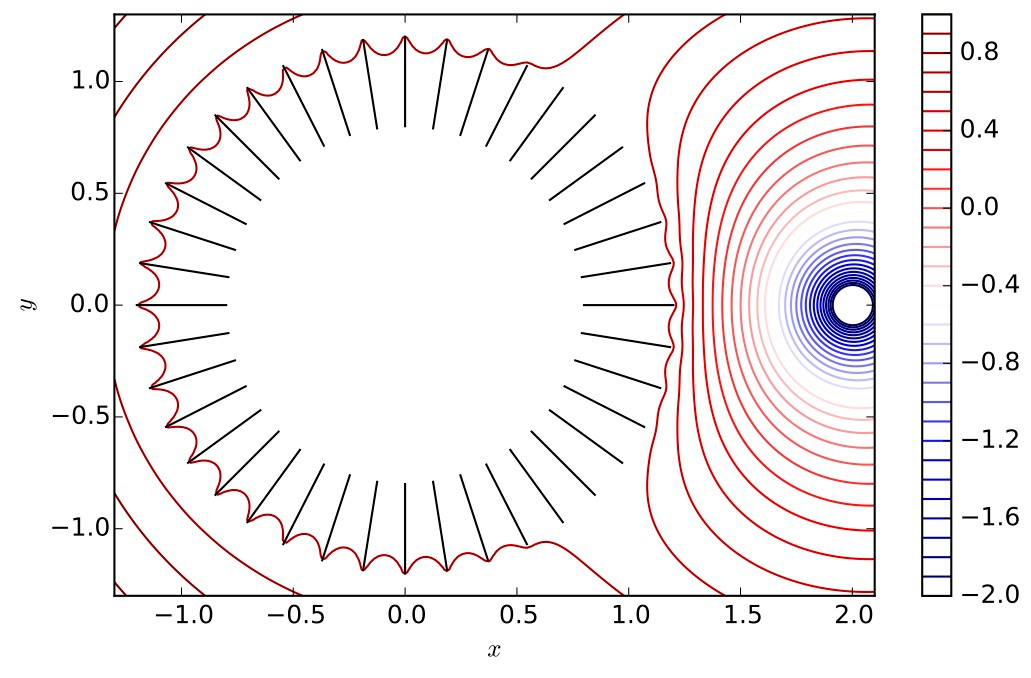
\includegraphics{Laplacetangentialplot.pdf}
\caption{Faradaycage}
\end{figure}


From the Green's function of the Laplacian, it is natural to consider logarithmic singular integrals over a contour

\[
L_\gamma f(z) = {1 \over \pi} \int_\gamma f(\zeta) \log|\zeta-z| \D s
\]
where $\D s$ is the arclength differential (as in line integrals, not complex analysis) and $f$ is real-valued. We focus on intervals where the arclength differential is just the standard one:

\[
L_{a,b} f(z) = {1 \over \pi }\int_a^b f(t) \log | z - t| \dt
\]
Note that off $[a,b]$, $u(x,y) \equiv u(x+\I y) = L f(x+\I y)$ solves Laplace's equation, and as the integrand has an integrable singularity it is continuous on $[a,b]$:


\begin{lstlisting}
(*@\HLJLk{using}@*) (*@\HLJLn{ApproxFun}@*)(*@\HLJLp{,}@*) (*@\HLJLn{SingularIntegralEquations}@*)(*@\HLJLp{,}@*) (*@\HLJLn{Plots}@*)
(*@\HLJLn{t}@*) (*@\HLJLoB{=}@*) (*@\HLJLnf{Fun}@*)(*@\HLJLp{()}@*)
(*@\HLJLn{f}@*) (*@\HLJLoB{=}@*) (*@\HLJLnf{sqrt}@*)(*@\HLJLp{(}@*)(*@\HLJLni{1}@*)(*@\HLJLoB{-}@*)(*@\HLJLn{t}@*)(*@\HLJLoB{{\textasciicircum}}@*)(*@\HLJLni{2}@*)(*@\HLJLp{)}@*)(*@\HLJLoB{*}@*)(*@\HLJLnf{exp}@*)(*@\HLJLp{(}@*)(*@\HLJLn{t}@*)(*@\HLJLp{)}@*)
(*@\HLJLn{u}@*) (*@\HLJLoB{=}@*) (*@\HLJLn{z}@*) (*@\HLJLoB{->}@*) (*@\HLJLnf{logkernel}@*)(*@\HLJLp{(}@*)(*@\HLJLn{f}@*)(*@\HLJLp{,}@*) (*@\HLJLn{z}@*)(*@\HLJLp{)}@*)  (*@\HLJLcs{{\#}}@*) (*@\HLJLcs{logkernel(f,z)}@*) (*@\HLJLcs{calculates}@*) (*@\HLJLcs{1/\ensuremath{\pi}}@*) (*@\HLJLcs{*}@*) (*@\HLJLcs{{\textbackslash}int}@*) (*@\HLJLcs{f(t)*log|t-z|}@*) (*@\HLJLcs{dt}@*)

(*@\HLJLn{xx}@*) (*@\HLJLoB{=}@*) (*@\HLJLn{yy}@*) (*@\HLJLoB{=}@*) (*@\HLJLoB{-}@*)(*@\HLJLni{2}@*)(*@\HLJLoB{:}@*)(*@\HLJLnfB{0.01}@*)(*@\HLJLoB{:}@*)(*@\HLJLni{2}@*)
(*@\HLJLn{U}@*) (*@\HLJLoB{=}@*) (*@\HLJLn{u}@*)(*@\HLJLoB{.}@*)(*@\HLJLp{(}@*)(*@\HLJLn{xx}@*)(*@\HLJLoB{{\textquotesingle}}@*) (*@\HLJLoB{.+}@*) (*@\HLJLn{im}@*)(*@\HLJLoB{*}@*)(*@\HLJLn{yy}@*)(*@\HLJLp{)}@*)

(*@\HLJLnf{contour}@*)(*@\HLJLp{(}@*)(*@\HLJLn{xx}@*)(*@\HLJLp{,}@*) (*@\HLJLn{yy}@*)(*@\HLJLp{,}@*) (*@\HLJLn{U}@*)(*@\HLJLp{)}@*)
(*@\HLJLnf{plot!}@*)(*@\HLJLp{(}@*)(*@\HLJLnf{domain}@*)(*@\HLJLp{(}@*)(*@\HLJLn{t}@*)(*@\HLJLp{);}@*) (*@\HLJLn{color}@*)(*@\HLJLoB{=:}@*)(*@\HLJLn{black}@*)(*@\HLJLp{,}@*) (*@\HLJLn{label}@*)(*@\HLJLoB{=}@*)(*@\HLJLs{"{}contour"{}}@*)(*@\HLJLp{)}@*)
\end{lstlisting}

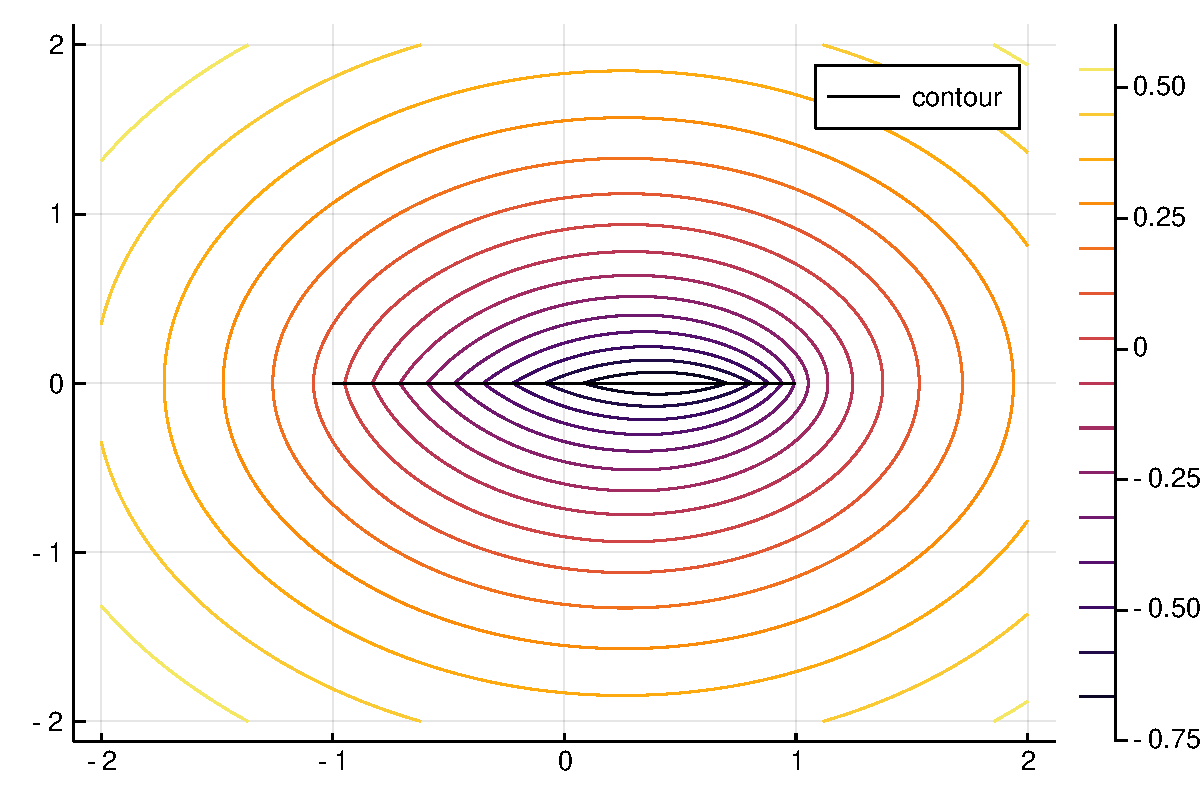
\includegraphics[width=\linewidth]{figures/Lecture17_1_1.pdf}

Or this can also be seen from a surface plot:


\begin{lstlisting}
(*@\HLJLnf{surface}@*)(*@\HLJLp{(}@*)(*@\HLJLn{xx}@*)(*@\HLJLp{,}@*) (*@\HLJLn{yy}@*)(*@\HLJLp{,}@*) (*@\HLJLn{U}@*)(*@\HLJLp{)}@*)
\end{lstlisting}

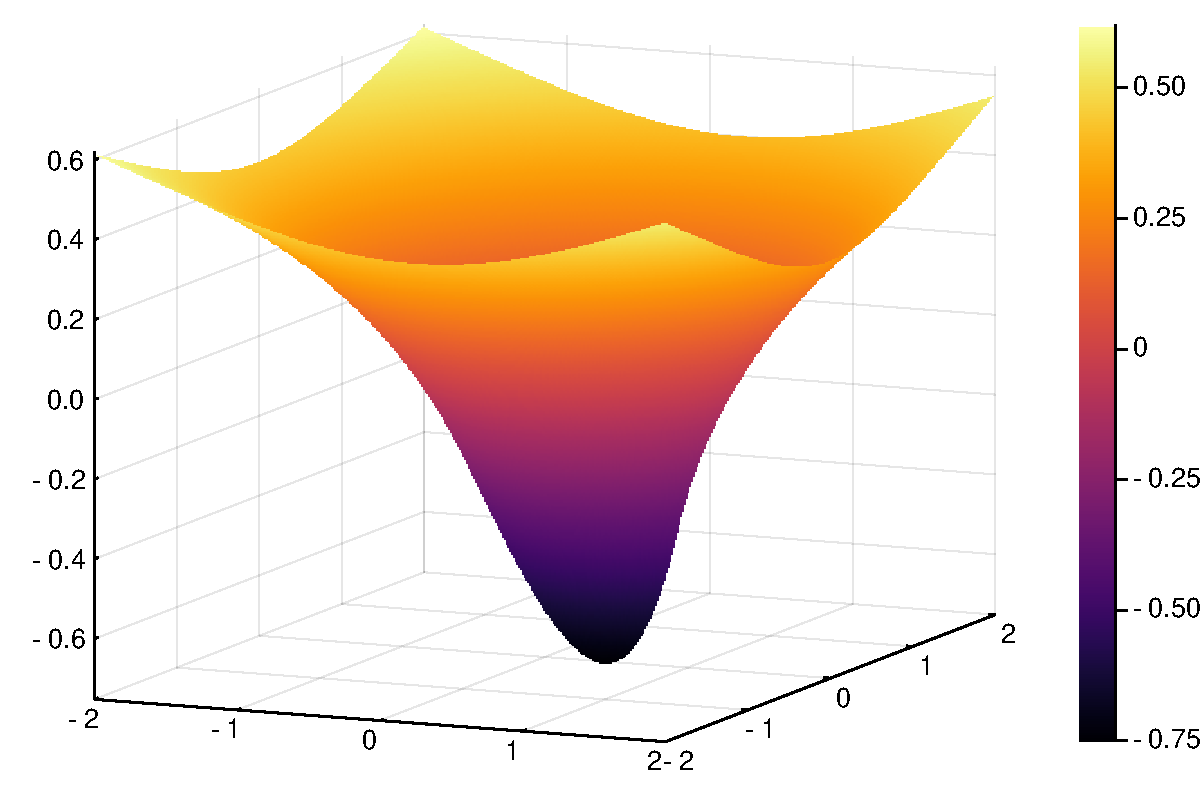
\includegraphics[width=\linewidth]{figures/Lecture17_2_1.pdf}

For $z \notin (-\infty,b]$ the fact that $u$ is harmonic (solves Laplace's equation)  can also be seen since $u$ is the real part of an analytic function:

\[
    u(z) = \Re Mf(z) \qqfor  Mf(z) := {1 \over \pi} \int_a^b f(t) \log ( z - t) \dt
\]
Note that the integrand avoids the branch cut of $\log z$. To extend this to $z\in (-\infty,a]$  (or more generally, $z \notin [a,\infty)$), we can use the alternative expression

\[
    u(z) = \Re \tilde Mf(z) \qqfor  \tilde Mf(z) := {1 \over \pi} \int_a^b f(t) \log ( t-z) \dt
\]
which follows from $\log|z-t| = \log|t-z|$.

\subsubsection{Evaluating logarithmic singular integrals}
To evaluate $L f(z)$ we evaluate $M f(z)$. Following our claim that the right way to represent analytic functions is by their behaviour at singularitites/branch cuts, we will accomplish this this by investigating the jumps of $M f(z)$. This allows us to reduce it to computing a Cauchy  transform.

\textbf{Lemma (Jumps of $M$)} Suppose $f$ satisfies the conditions of Plemelj. Then $M f(z)$ satisfies the following

\begin{itemize}
\item[1. ] Analyticity: $M$ is analytic off $(-\infty,b]$


\item[2. ] Regularity: $M$ has weaker than pole singularities


\item[3. ] Asymptotics: 

\end{itemize}
\[
Mf(z) = {1 \over \pi} \int_a^b f(t) \D t \log z + o(1) \qqas z \rightarrow \infty
\]
\begin{itemize}
\item[4. ] Jump: for $x < a$ we have

\end{itemize}
\[
M^+f(x) - M^-f(x) = 2 \I \int_a^b f(t) \D t
\]
and for $a < x < b$ we have

\[
M^+ f(x) - M^-f(x) = 2 \I \int_x^b f(t) \D t
\]
\textbf{Proof}

Analyticity property (1) follows immediately from definition: we have for $z \notin (-\infty,b]$

\[
{\D \over \D z} M f(z) = {1 \over \pi} \int_{-1}^1 f(t) {1\over z -t}  \dt = -2 \I \CC f(z)
\]
The regularity property (2) follows from the expression as an antiderivative: we know $\CC f(z)$ has weaker than pole singularities and integrating only makes them better. To derive the asymptotics (3) we use

\[
\log(z - t) = \log z + \log(1 - t/z)
\]
Finally we get to the jumps. For any point $c > b$ we write 

\[
M f(z) = -2 \I \int_c^z \CC f(\zeta) \D \zeta + M f(c)
\]
For $x < a$ we can deform the contour just above/below the interval giving us

\[
M^\pm f(x) = Mf(c) -2 \I \int_c^b \CC f(t) \D t -2 \I \int_b^a \CC^\pm f(t) \D t -2 \I \int_a^x \CC f(t) \D t
\]
so that

\[
(M^+ - M^-) f(x) = -2 \I \int_b^a (\CC^+ - \CC^-) f(t) \D t  = 2 \I \int_a^b f(t) \D t
\]
Similarly for $a < x < b$ we have

\[
M^\pm f(x) = Mf(c) -2 \I \int_c^b \CC f(t) \D t -2 \I \int_b^x \CC^\pm f(t) \D t 
\]
which gives

\[
(M^+ - M^-) f(x) = -2 \I \int_b^x (\CC^+ - \CC^-) f(t) \D t  = 2 \I \int_x^b f(t) \D t.
\]
\ensuremath{\blacksquare}

We can construct a function that satisfies the same 4 properties using the Cauchy transform. By uniqueness they must be the same.

\textbf{Theorem (Log kernel as Cauchy)}  Suppose $f$ satisfies the conditions of Plemelj and define the (negative) indefinite integral of $f$ via 

\[
F(x) := \int_x^b f(t) \D t.
\]
Then

\[
M f(z) = {\log(z-a) \over \pi} \int_a^b f(t) \D t + 2 \I \CC F(z)
\]
\textbf{Proof}

Define

\[
\phi(z) := {\log(z-a) \over \pi} \int_a^b f(t) \D t + 2 \I \CC F(z)
\]
This satisfies conditions (1\ensuremath{\endash}4) above. Therefore $\phi(z) - M f(z)$ is continuous hence analytic on $(-\infty,a)$ and $(a,b)$, has weaker than pole singularities at $a$ and $b$ so analytic there too: it is entire. The logarithmic growth at infinity cancels therefore it is zero by Liouville.

\ensuremath{\blacksquare}



\end{document}
